\documentclass[9pt,a4paper]{article}
\usepackage[margin=15mm]{geometry}
\usepackage[T1]{fontenc}
\usepackage{lmodern}
\usepackage{microtype}
\usepackage{graphicx}
\usepackage{float}
\usepackage{booktabs}
\usepackage{amsmath}
\usepackage{xcolor}
\usepackage{listings}
\usepackage{hyperref}
\usepackage{enumitem}
\usepackage{caption}
\usepackage{subcaption}
\usepackage{titlesec}

\setlength{\parindent}{0pt}
\setlength{\parskip}{3pt}
\setlist{nosep,leftmargin=*}
\captionsetup{font=small,skip=2pt}
\hypersetup{colorlinks=true,urlcolor=blue!55!black,linkcolor=blue!55!black}
\definecolor{sectionblue}{HTML}{1F4E79}
\definecolor{titlered}{HTML}{8B0000}
\definecolor{vscodeblue}{HTML}{569CD6}
\definecolor{vscodecyan}{HTML}{4EC9B0}
\definecolor{vscodegreen}{HTML}{6A9955}
\definecolor{vscodeorange}{HTML}{CE9178}
\definecolor{vscodepurple}{HTML}{C586C0}
\definecolor{vscodegray}{HTML}{6A737D}
\titleformat{\section}{\color{sectionblue}\large\bfseries}{\thesection}{0.6em}{}
\lstset{
  basicstyle=\color{vscodegray}\ttfamily\scriptsize,
  keywordstyle=\color{vscodeblue}\bfseries,
  commentstyle=\color{vscodegreen},
  stringstyle=\color{vscodeorange},
  identifierstyle=\color{vscodecyan},
  emph={True,False,None,def,class,return,import,from,as,for,in},
  emphstyle=\color{vscodepurple},
  breaklines=true, frame=single, rulecolor=\color{vscodegray}, numbers=none,
  showstringspaces=false, xleftmargin=3pt, xrightmargin=3pt,
  aboveskip=3pt, belowskip=3pt
}
\newcommand{\resultfigure}[2]{%
  \begin{figure}[H]\centering
  \IfFileExists{#1}{\includegraphics[width=0.76\linewidth,height=0.15\textheight,keepaspectratio]{#1}}%
  {\fbox{\parbox[c][22mm][c]{0.72\linewidth}{\centering Missing image: \texttt{\detokenize{#1}}}}}
  \caption{#2}
  \end{figure}
}
\newcommand{\resultfiguregrid}[8]{%
  \begin{figure}[H]\centering
  \subcaptionbox{#2\label{fig:grid-a}}[0.48\linewidth]{%
    \IfFileExists{#1}{\includegraphics[width=\linewidth,height=0.17\textheight,keepaspectratio]{#1}}%
    {\fbox{\parbox[c][22mm][c]{0.9\linewidth}{\centering Missing image: \texttt{\detokenize{#1}}}}}}%
  \hfill
  \subcaptionbox{#4\label{fig:grid-b}}[0.48\linewidth]{%
    \IfFileExists{#3}{\includegraphics[width=\linewidth,height=0.17\textheight,keepaspectratio]{#3}}%
    {\fbox{\parbox[c][22mm][c]{0.9\linewidth}{\centering Missing image: \texttt{\detokenize{#3}}}}}}\\[4pt]
  \subcaptionbox{#6\label{fig:grid-c}}[0.48\linewidth]{%
    \IfFileExists{#5}{\includegraphics[width=\linewidth,height=0.17\textheight,keepaspectratio]{#5}}%
    {\fbox{\parbox[c][22mm][c]{0.9\linewidth}{\centering Missing image: \texttt{\detokenize{#5}}}}}}%
  \hfill
  \subcaptionbox{#8\label{fig:grid-d}}[0.48\linewidth]{%
    \IfFileExists{#7}{\includegraphics[width=\linewidth,height=0.17\textheight,keepaspectratio]{#7}}%
    {\fbox{\parbox[c][22mm][c]{0.9\linewidth}{\centering Missing image: \texttt{\detokenize{#7}}}}}}%
  \caption{ResNet18 training results.}
  \end{figure}
}
\newcommand{\resultfigurerow}[4]{%
  \begin{figure}[H]\centering
  \subcaptionbox{#2}[0.48\linewidth]{%
    \IfFileExists{#1}{\includegraphics[width=\linewidth,height=0.17\textheight,keepaspectratio]{#1}}%
    {\fbox{\parbox[c][22mm][c]{0.9\linewidth}{\centering Missing image: \texttt{\detokenize{#1}}}}}}%
  \hfill
  \subcaptionbox{#4}[0.48\linewidth]{%
    \IfFileExists{#3}{\includegraphics[width=\linewidth,height=0.17\textheight,keepaspectratio]{#3}}%
    {\fbox{\parbox[c][22mm][c]{0.9\linewidth}{\centering Missing image: \texttt{\detokenize{#3}}}}}}%
  \caption{ResNet18 training results.}
  \end{figure}
}
\newcommand{\resultfigurerowcontinued}[4]{%
  \begin{figure}[H]\ContinuedFloat\centering
  \subcaptionbox{#2}[0.48\linewidth]{%
    \IfFileExists{#1}{\includegraphics[width=\linewidth,height=0.17\textheight,keepaspectratio]{#1}}%
    {\fbox{\parbox[c][22mm][c]{0.9\linewidth}{\centering Missing image: \texttt{\detokenize{#1}}}}}}%
  \hfill
  \subcaptionbox{#4}[0.48\linewidth]{%
    \IfFileExists{#3}{\includegraphics[width=\linewidth,height=0.17\textheight,keepaspectratio]{#3}}%
    {\fbox{\parbox[c][22mm][c]{0.9\linewidth}{\centering Missing image: \texttt{\detokenize{#3}}}}}}%
  \caption{ResNet18 training results (continued).}
  \end{figure}
}
\title{\vspace{-1.2cm}\textcolor{titlered}{\textbf{EN3160 -- Assignment 3: Neural Networks}}}
\author{Saruka U. \quad | \quad Index Number: 230585C\\
\small GitHub: \url{https://github.com/Saruka03/EN3160-Assignment-03}}
\date{}
\begin{document}
\maketitle
\vspace{-1.2cm}

\section*{Task 1 -- Manually Implemented Dense Network}
The CIFAR-10 network was modified to include a hidden layer with 100 neurons and sigmoid activation. Cross-entropy loss was used, and forward propagation, backpropagation, and parameter updates were implemented manually. The network was trained for 10 epochs.

\textbf{Core architecture (PyTorch-style notation):}
\begin{lstlisting}[language=Python, caption={Manual forward and backward pass for Task 1}]
# Network: input -> 100 sigmoid units -> 10 classes
hidden = torch.sigmoid(x_train @ W1 + b1)
logits = hidden @ W2 + b2

# Cross-entropy from logits (labels contain class indices)
probs = torch.softmax(logits, dim=1)
loss = -torch.log_softmax(logits, dim=1)[
    torch.arange(len(labels)), labels
].mean()

# Manual gradients: softmax + cross-entropy
dlogits = probs.clone()
dlogits[torch.arange(len(labels)), labels] -= 1
dlogits /= len(labels)

dW2 = hidden.T @ dlogits
db2 = dlogits.sum(dim=0)

dhidden = dlogits @ W2.T
dhidden *= hidden * (1 - hidden)  # sigmoid derivative

dW1 = x_train.T @ dhidden
db1 = dhidden.sum(dim=0)

# Manual parameter updates
W1 -= learning_rate * dW1
b1 -= learning_rate * db1
W2 -= learning_rate * dW2
b2 -= learning_rate * db2
\end{lstlisting}

The training and test loss decreased throughout training. After 10 epochs, training and test accuracy reached 39.71\%.

\begin{table}[H]\centering
\caption{Task 1 results after 10 epochs.}
\begin{tabular}{lc}\toprule
Metric & Accuracy\\\midrule
Training & 39.71\%\\
Test & 39.71\%\\\bottomrule
\end{tabular}
\end{table}
The similar training and test accuracies indicate comparable performance on both datasets. However, the overall accuracy remains modest, suggesting that the manually implemented dense network has limited classification capability for CIFAR-10 images.

\resultfigure{../notebooks/results/task1_plots.png}{Training and test cross-entropy loss and accuracy over 10 epochs.}

% --------------------------------------------------
% Task 2: CNN Classification on MNIST
% --------------------------------------------------
\section*{Task 2 -- CNN Classification on MNIST}

LeNet-5 and a modern three-layer CNN were trained on the
MNIST dataset for 10 epochs using cross-entropy loss.
The modern CNN incorporates batch normalization and
dropout to improve training stability and reduce
overfitting.
\begin{lstlisting}[language=Python, basicstyle=\ttfamily\scriptsize, caption={LeNet-5 architecture for MNIST}]
self.features = nn.Sequential(
    nn.Conv2d(1, 6, 5), nn.Tanh(),
    nn.AvgPool2d(2),
    nn.Conv2d(6, 16, 5), nn.Tanh(),
    nn.AvgPool2d(2)
)
self.classifier = nn.Sequential(
    nn.Linear(16*4*4, 120), nn.Tanh(),
    nn.Linear(120, 84), nn.Tanh(),
    nn.Linear(84, 10)
)
\end{lstlisting}

\begin{lstlisting}[language=Python, basicstyle=\ttfamily\scriptsize, caption={Modern CNN architecture for MNIST}]
nn.Sequential(
    nn.Conv2d(1, 32, 3, padding=1),
    nn.BatchNorm2d(32), nn.ReLU(),
    nn.MaxPool2d(2), nn.Dropout2d(0.25),
    nn.Conv2d(32, 64, 3, padding=1),
    nn.BatchNorm2d(64), nn.ReLU(),
    nn.MaxPool2d(2), nn.Dropout2d(0.25),
    nn.Conv2d(64, 128, 3, padding=1),
    nn.BatchNorm2d(128), nn.ReLU(),
    nn.MaxPool2d(2), nn.Dropout2d(0.25)
)
self.classifier = nn.Sequential(
    nn.Flatten(),
    nn.Linear(128*3*3, 128), nn.ReLU(),
    nn.Dropout(0.5), nn.Linear(128, 10)
)
\end{lstlisting}

\textbf{Results after 10 Epochs}

\begin{table}[htbp]
\centering
\caption{Performance comparison of LeNet-5 and Modern CNN.}
\label{tab:mnist_results}
\small
\begin{tabular}{lrrrr}
\toprule
\textbf{Model} &
\textbf{Train Acc. (\%)} &
\textbf{Test Acc. (\%)} &
\textbf{Train Loss} &
\textbf{Test Loss} \\
\midrule
LeNet-5
& 99.4017 & 98.6000 & 0.0184 & 0.0412 \\
Modern CNN
& 99.6467 & 99.1700 & 0.0108 & 0.0272 \\
\bottomrule
\end{tabular}
\end{table}

The modern CNN achieved a test accuracy of 99.17\%,
outperforming LeNet-5 by 0.57 percentage points.
It also achieved lower training and test losses.
The training--test accuracy gap decreased from
0.80 percentage points for LeNet-5 to 0.48 percentage
points for the modern CNN. These results indicate
better classification performance on the MNIST test set.

\textbf{Confusion Matrices}

Figure~\ref{fig:mnist_comparison} compares the per-epoch
training and test accuracy and cross-entropy loss of
both models over 10 epochs. Figure~\ref{fig:mnist_confusion}
presents the test-set confusion matrices for both models.
These matrices show the distribution of correct classifications
and misclassifications across the ten digit classes.

\begin{figure}[H]
    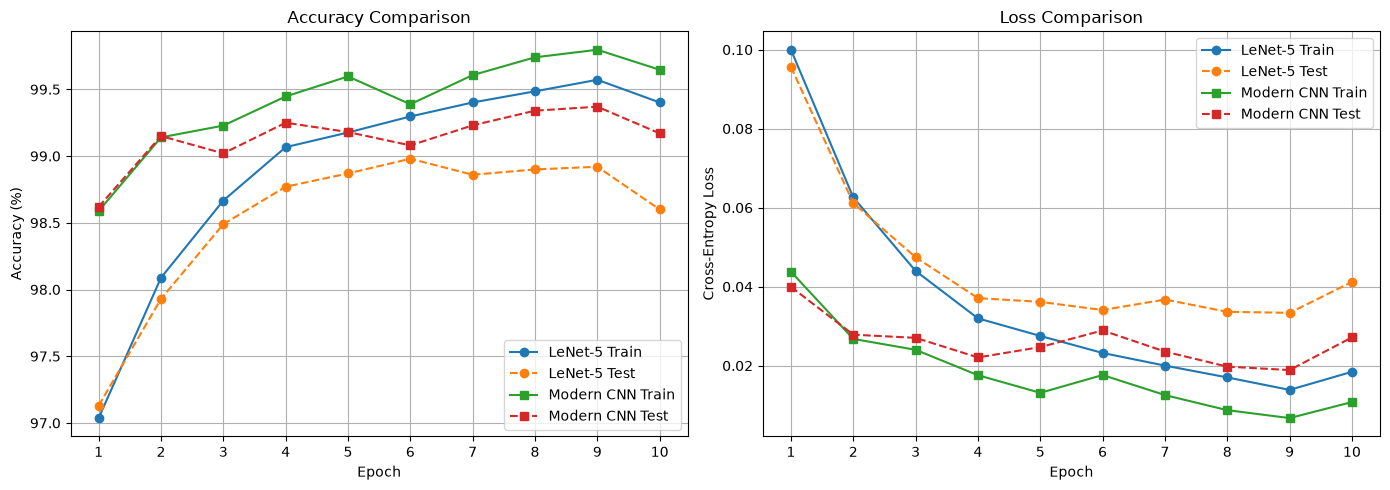
\includegraphics[width=0.98\linewidth]
    {../notebooks/results/task2_comparison.png}
    \caption{Per-epoch training and test accuracy and
    cross-entropy loss comparison between LeNet-5 and
    the Modern CNN.}
    \label{fig:mnist_comparison}
\end{figure}

\begin{figure}[H]
    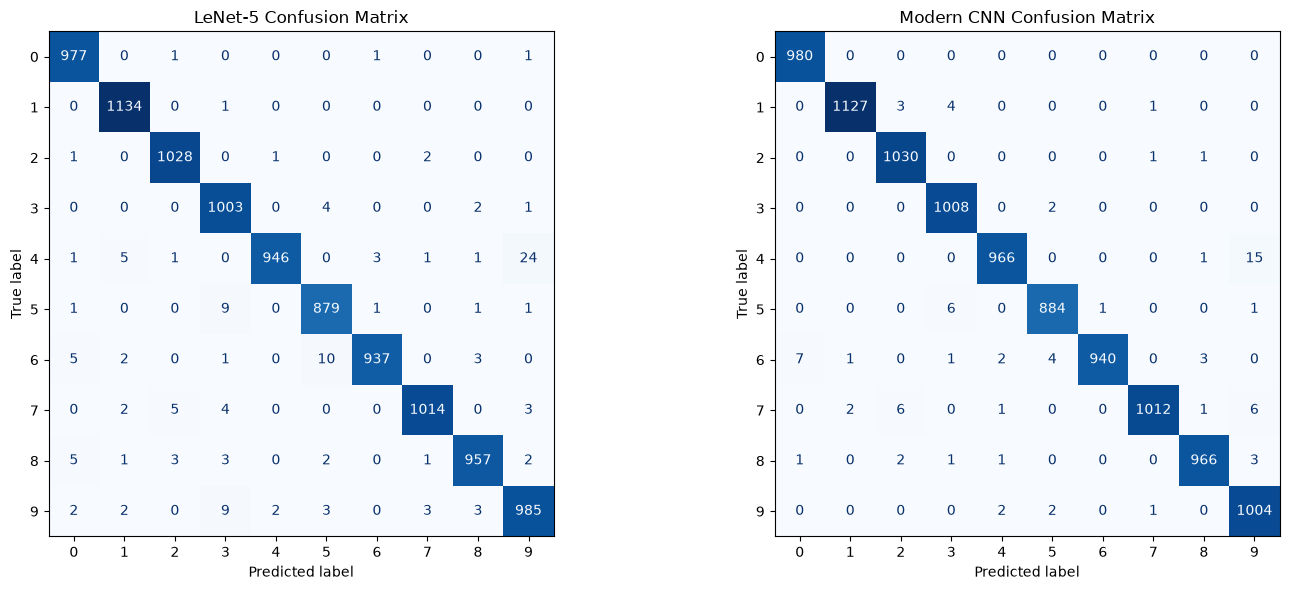
\includegraphics[width=0.85\linewidth]
    {../notebooks/results/task2_confusion_matrices.png}
    \caption{Test-set confusion matrices for LeNet-5
    and the Modern CNN.}
    \label{fig:mnist_confusion}
\end{figure}

\section*{Task 3 -- Transfer Learning with ResNet18}
ImageNet-1K-pretrained ResNet18 was adapted to classify ants and bees. Images were resized to \(224\times224\) and normalized using ImageNet statistics. For fine-tuning, all model parameters were trainable. For feature extraction, the pretrained backbone was frozen and only the final classifier was trained.

\textbf{Key implementation:}
\begin{lstlisting}[language=Python]
model = models.resnet18(weights=models.ResNet18_Weights.DEFAULT)
for p in model.parameters():
    p.requires_grad = False       # feature extraction
model.fc = nn.Linear(model.fc.in_features, 2)
optimizer = optim.SGD(
    filter(lambda p: p.requires_grad, model.parameters()),
    lr=0.001, momentum=0.9
)
\end{lstlisting}

\begin{table}[H]\centering
\caption{Recorded Hymenoptera results.}
\begin{tabular}{lcc}\toprule
Method & Final train acc. & Best validation acc.\\\midrule
Fine-tuning & 99.59\% & 94.77\%\\
Feature extraction & 94.26\% & 94.12\%\\\bottomrule
\end{tabular}
\end{table}
Fine-tuning had slightly higher best validation accuracy in this run. The difference is small, and the validation set is limited, so it should not be treated as evidence that fine-tuning will always be better.

\resultfigurerow
  {../notebooks/results/task3_fine-tuning_accuracy.png}{ResNet18 fine-tuning accuracy.}
  {../notebooks/results/task3_fine-tuning_loss.png}{ResNet18 fine-tuning loss.}
\clearpage
\resultfigurerowcontinued
  {../notebooks/results/task3_feature_extraction_accuracy.png}{ResNet18 feature-extraction accuracy.}
  {../notebooks/results/task3_feature_extraction_loss.png}{ResNet18 feature-extraction loss.}

\section*{Conclusion}
The manually implemented CIFAR-10 network achieved 39.71\% test accuracy. On MNIST, the modern CNN outperformed LeNet-5 with 99.17\% test accuracy versus 98.60\%. On Hymenoptera, ResNet18 fine-tuning achieved 94.77\% best validation accuracy, while feature extraction achieved 94.12\%. The modern CNN was the strongest of the tested MNIST models; both transfer-learning methods performed similarly on the small validation set.

\end{document}
